\section{Predicting Temperature Time Series with LSTM Using
PyTorch}\label{predicting-temperature-time-series-with-lstm-using-pytorch}

\subsubsection{Introduction}\label{introduction}

Long Short-Term Memory (LSTM) is a type of recurrent neural network
(RNN) that is commonly used for sequence modeling, particularly for
processing time-series data. Unlike traditional RNNs, LSTMs have a
memory cell that allows them to selectively remember or forget
information over time, which makes them particularly useful for
long-term dependencies.

In this tutorial, we'll use Pytorch to build an LSTM model that can
predict a time-series based on previous data. We'll use numpy and pandas
to preprocess the data.

\subsection{Step 1: Import Libraries}\label{step-1-import-libraries}

We'll start by importing the necessary libraries.

\begin{lstlisting}[language=Python]
import numpy as np
import pandas as pd
import torch
import torch.nn as nn
\end{lstlisting}

\begin{lstlisting}
/opt/venv/lib/python3.10/site-packages/tqdm/auto.py:21: TqdmWarning: IProgress not found. Please update jupyter and ipywidgets. See https://ipywidgets.readthedocs.io/en/stable/user_install.html
  from .autonotebook import tqdm as notebook_tqdm
\end{lstlisting}

\subsubsection{Step 2: Load Data}\label{step-2-load-data}

For this tutorial, we'll use a sample dataset that contains temperature
readings for a single sensor over time. We'll load the dataset into a
pandas DataFrame and preprocess it so that it can be fed into our LSTM
model.

\begin{lstlisting}[language=Python]
# Load data into a pandas DataFrame
df = pd.read_csv('../data/temperature.csv')

# Convert the 'datetime' column to a datetime object
df['Date'] = pd.to_datetime(df['Date'])

# Set the 'datetime' column as the index
df.set_index('Date', inplace=True)

# Resample the data to hourly intervals and fill missing values with the previous value
df = df.resample('H').ffill()

# Normalize the data
df = (df - df.mean()) / df.std()

# Convert the DataFrame to a numpy array
data = df.values
\end{lstlisting}

\subsubsection{Step 3: Split Data}\label{step-3-split-data}

Next, we'll split the data into training and testing sets. We'll use the
first 70\% of the data for training and the remaining 30\% for testing.

\begin{lstlisting}[language=Python]
# Split the data into training and testing sets
train_size = int(len(data) * 0.7)
train_data, test_data = data[:train_size], data[train_size:]
\end{lstlisting}

\subsubsection{Step 4: Create Data
Sequences}\label{step-4-create-data-sequences}

Before we can train our LSTM model, we need to create sequences of data
that the model can learn from. We'll create sequences of length 24 (one
day), and we'll use a sliding window approach to create overlapping
sequences.

\begin{lstlisting}[language=Python]
# Function to create sequences of data
def create_sequences(data, seq_length):
    X = []
    y = []
    for i in range(len(data) - seq_length):
        X.append(data[i:i+seq_length])
        y.append(data[i+seq_length])
    return np.array(X), np.array(y)

# Create sequences for training and testing data
seq_length = 24
X_train, y_train = create_sequences(train_data, seq_length)
X_test, y_test = create_sequences(test_data, seq_length)
\end{lstlisting}

\subsubsection{Step 5: Create LSTM
Model}\label{step-5-create-lstm-model}

Now, we'll create our LSTM model using Pytorch. Our model will have one
LSTM layer with 32 hidden units and one fully connected output layer.

\begin{lstlisting}[language=Python]
class LSTM(nn.Module):
    def __init__(self, input_size, hidden_size, output_size):
        super(LSTM, self).__init__()
        self.lstm = nn.LSTM(input_size, hidden_size, batch_first=True)
        self.fc = nn.Linear(hidden_size, output_size)

    def forward(self, x):
        out, _ = self.lstm(x)
        out = self.fc(out[:, -1, :])
        return out
\end{lstlisting}

In the \lstinline{\_\_init\_\_} method, we define an LSTM
layer with hidden\_size hidden units and a fully connected output layer
with output\_size output units. In the forward method, we pass the input
\lstinline{x} through the LSTM layer, take the output of
the last time step, and pass it through the fully connected output
layer.

\subsubsection{Step 6: Instantiate Model and Define Loss Function and
Optimizer}\label{step-6-instantiate-model-and-define-loss-function-and-optimizer}

Now, we'll instantiate our LSTM model, define our loss function (mean
squared error), and define our optimizer (Adam).

\begin{lstlisting}[language=Python]
# Instantiate the model
input_size = X_train.shape[2]
hidden_size = 32
output_size = 1
model = LSTM(input_size, hidden_size, output_size)

# Define the loss function and optimizer
criterion = nn.MSELoss()
optimizer = torch.optim.Adam(model.parameters(), lr=0.001)
\end{lstlisting}

\subsubsection{Step 7: Train the Model}\label{step-7-train-the-model}

Next, we'll train our LSTM model on the training data. We'll use a batch
size of 32 and train for 50 epochs.

\begin{lstlisting}[language=Python]
# Convert numpy arrays to Pytorch tensors
X_train = torch.from_numpy(X_train).float()
y_train = torch.from_numpy(y_train).float()
X_test = torch.from_numpy(X_test).float()
y_test = torch.from_numpy(y_test).float()

# Define the batch size and number of epochs
batch_size = 32
num_epochs = 25

# Train the model
for epoch in range(num_epochs):
    # Shuffle the training data
    perm = torch.randperm(X_train.shape[0])
    X_train = X_train[perm]
    y_train = y_train[perm]

    # Loop over batches
    for i in range(0, X_train.shape[0], batch_size):
        # Get batch
        batch_X = X_train[i:i+batch_size]
        batch_y = y_train[i:i+batch_size]

        # Zero the gradients
        optimizer.zero_grad()

        # Forward pass
        outputs = model(batch_X)
        loss = criterion(outputs, batch_y)

        # Backward pass and optimization
        loss.backward()
        optimizer.step()

    # Print loss for this epoch
    print('Epoch [{}/{}], Loss: {:.4f}'.format(epoch+1, num_epochs, loss.item()))
\end{lstlisting}

\begin{lstlisting}
Epoch [1/25], Loss: 3.4126
Epoch [2/25], Loss: 0.0009
Epoch [3/25], Loss: 0.0003
Epoch [4/25], Loss: 0.0001
Epoch [5/25], Loss: 0.0001
Epoch [6/25], Loss: 0.0010
Epoch [7/25], Loss: 0.0367
Epoch [8/25], Loss: 0.0002
Epoch [9/25], Loss: 0.1150
Epoch [10/25], Loss: 0.0002
Epoch [11/25], Loss: 0.0001
Epoch [12/25], Loss: 0.0003
Epoch [13/25], Loss: 0.0000
Epoch [14/25], Loss: 0.0000
Epoch [15/25], Loss: 0.0001
Epoch [16/25], Loss: 0.0013
Epoch [17/25], Loss: 0.0000
Epoch [18/25], Loss: 0.0006
Epoch [19/25], Loss: 0.0000
Epoch [20/25], Loss: 0.0000
Epoch [21/25], Loss: 0.0000
Epoch [22/25], Loss: 0.0009
Epoch [23/25], Loss: 0.0005
Epoch [24/25], Loss: 0.0000
Epoch [25/25], Loss: 0.0000
\end{lstlisting}

\subsubsection{Step 8: Evaluate the
Model}\label{step-8-evaluate-the-model}

Finally, we'll evaluate our LSTM model on the testing data.

\begin{lstlisting}[language=Python]
# Evaluate the model on the test data
model.eval()
with torch.no_grad():
    y_pred = model(X_test)

# Calculate the test loss
test_loss = criterion(y_pred, y_test)
print('Test Loss: {:.4f}'.format(test_loss.item()))
\end{lstlisting}

\begin{lstlisting}
Test Loss: 0.0167
\end{lstlisting}

\begin{lstlisting}[language=Python]
import matplotlib.pyplot as plt

# Convert Pytorch tensors to numpy arrays
y_test = y_test.numpy()
y_pred = y_pred.numpy()

# Plot predicted vs actual values
plt.figure(figsize=(10, 6))
plt.plot(y_test[:500], label='Actual')
plt.plot(y_pred[:500], label='Predicted')
plt.xlabel('Time Step')
plt.ylabel('Value')
plt.title('LSTM Predictions')
plt.legend()
plt.show()
\end{lstlisting}

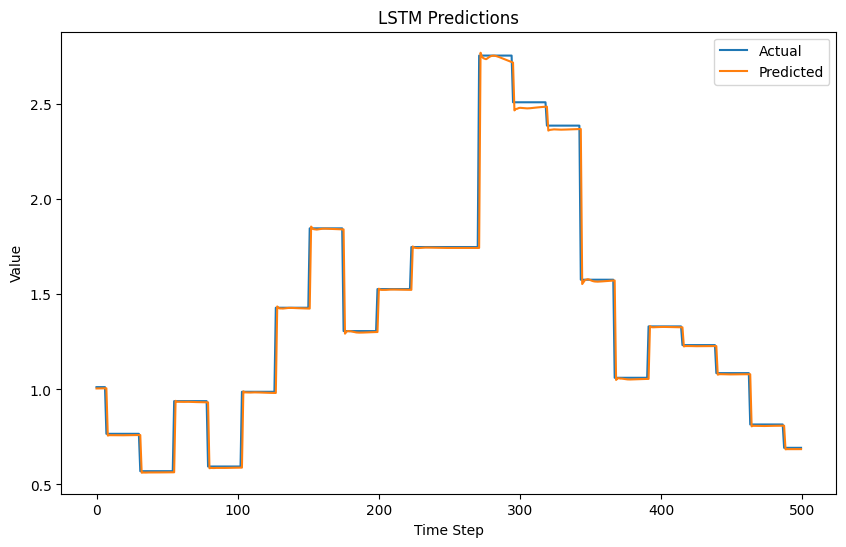
\includegraphics{img/rnn/lstm/output_16_0_pred_temp.png}

